\documentclass[12pt,a4paper]{article}
\usepackage[utf8]{inputenc}
\usepackage[greek, english]{babel} 
\usepackage{alphabeta}
\usepackage{amsmath}
\usepackage{amssymb}
\usepackage{graphicx}
\usepackage{listings}
\usepackage{xcolor}
\usepackage{tikz}
\usetikzlibrary{automata,positioning,arrows.meta,shapes.geometric}
\usepackage{float}
\usepackage{geometry}
\usepackage{hyperref}
\usepackage{booktabs}
\usepackage{array}
\usepackage{caption}
\usepackage{subcaption}
\usepackage{fancyhdr}
\usepackage{lastpage}

\geometry{margin=2.5cm}

% Διόρθωση για το warning του fancyhdr
\setlength{\headheight}{15pt}

% Ρυθμίσεις για listings (κώδικας Verilog)
\definecolor{codegreen}{rgb}{0,0.6,0}
\definecolor{codegray}{rgb}{0.5,0.5,0.5}
\definecolor{codepurple}{rgb}{0.58,0,0.82}
\definecolor{backcolour}{rgb}{0.95,0.95,0.92}

% Χαρτογράφηση ελληνικών χαρακτήρων για το listings
\lstset{
    inputencoding=utf8,
    extendedchars=true,
    literate={Α}{{\textAlpha}}1 {Β}{{\textBeta}}1 {Γ}{{\textGamma}}1 {Δ}{{\textDelta}}1 {Ε}{{\textEpsilon}}1 {Ζ}{{\textZeta}}1 {Η}{{\textEta}}1 {Θ}{{\textTheta}}1 {Ι}{{\textIota}}1 {Κ}{{\textKappa}}1 {Λ}{{\textLambda}}1 {Μ}{{\textMu}}1 {Ν}{{\textNu}}1 {Ξ}{{\textXi}}1 {Ο}{{\textOmicron}}1 {Π}{{\textPi}}1 {Ρ}{{\textRho}}1 {Σ}{{\textSigma}}1 {Τ}{{\textTau}}1 {Υ}{{\textUpsilon}}1 {Φ}{{\textPhi}}1 {Χ}{{\textChi}}1 {Ψ}{{\textPsi}}1 {Ω}{{\textOmega}}1
    {α}{{\textalpha}}1 {β}{{\textbeta}}1 {γ}{{\textgamma}}1 {δ}{{\textdelta}}1 {ε}{{\textepsilon}}1 {ζ}{{\textzeta}}1 {η}{{\texteta}}1 {θ}{{\texttheta}}1 {ι}{{\textiota}}1 {κ}{{\textkappa}}1 {λ}{{\textlambda}}1 {μ}{{\textmu}}1 {ν}{{\textnu}}1 {ξ}{{\textxi}}1 {ο}{{\textomicron}}1 {π}{{\textpi}}1 {ρ}{{\textrho}}1 {σ}{{\textsigma}}1 {ς}{{\textsigma}}1 {τ}{{\texttau}}1 {υ}{{\textupsilon}}1 {φ}{{\textphi}}1 {χ}{{\textchi}}1 {ψ}{{\textpsi}}1 {ω}{{\textomega}}1
    {ά}{{\'a}}1 {έ}{{\'e}}1 {ή}{{\'h}}1 {ί}{{\'i}}1 {ό}{{\'o}}1 {ύ}{{\'u}}1 {ώ}{{\'w}}1
}

\lstdefinestyle{verilogstyle}{
    backgroundcolor=\color{backcolour},
    commentstyle=\color{codegreen},
    keywordstyle=\color{blue}\bfseries,
    numberstyle=\tiny\color{codegray},
    stringstyle=\color{codepurple},
    basicstyle=\ttfamily\footnotesize,
    breakatwhitespace=false,
    breaklines=true,
    captionpos=b,
    keepspaces=true,
    numbers=left,
    numbersep=5pt,
    showspaces=false,
    showstringspaces=false,
    showtabs=false,
    tabsize=2,
    frame=single,
    language=Verilog
}

\lstset{style=verilogstyle}

% Header/Footer
\pagestyle{fancy}
\fancyhf{}
\rhead{Ψηφιακά Συστήματα HW-1}
\lhead{Εργαστηριακές Ασκήσεις}
\rfoot{Σελίδα \thepage\ από \pageref{LastPage}}

\title{
    \vspace{5cm}
    \textbf{Ψηφιακά Συστήματα HW σε Χαμηλά Επίπεδα Λογικής I}\\
    \vspace{1cm}
    \Large Αναφορά Εργαστηριακών Ασκήσεων  
    Εξοικείωσης με τη Verilog\\
    \vspace{10cm}
}
\author{
    \textbf{Ζωίδης Βασίλειος}\\
    ΑΕΜ: \textbf{10652}
}
\date{Ιανουάριος 2026}

\begin{document}

\maketitle
\newpage
\thispagestyle{fancy}

\tableofcontents
\newpage

%==============================================================================
\section{Εισαγωγή}
%==============================================================================

Η παρούσα αναφορά περιγράφει την υλοποίηση τεσσάρων εργαστηριακών ασκήσεων σε γλώσσα Verilog, με στόχο τη σχεδίαση ενός απλού AI accelerator. Οι ασκήσεις περιλαμβάνουν:

\begin{enumerate}
    \item Σχεδίαση μιας Αριθμητικής/Λογικής Μονάδας (ALU) 32-bit
    \item Υλοποίηση αριθμομηχανής με χρήση της ALU
    \item Δημιουργία Register File με πολλαπλές θύρες ανάγνωσης/εγγραφής
    \item Σχεδίαση νευρωνικού δικτύου με FSM
\end{enumerate}

Η προσομοίωση πραγματοποιήθηκε στο Playground EDA.

%==============================================================================
\section{Άσκηση 1: Αριθμητική/Λογική Μονάδα (ALU)}
%==============================================================================

\subsection{Περιγραφή}

Η ALU είναι ένα συνδυαστικό κύκλωμα 32-bit που υλοποιεί τις ακόλουθες λειτουργίες:

\begin{table}[H]
\centering
\caption{Πίνακας λειτουργιών ALU}
\begin{tabular}{|c|l|}
\hline
\textbf{alu\_op} & \textbf{Λειτουργία} \\
\hline
1000 & Λογική AND \\
1001 & Λογική OR \\
1010 & Λογική NOR \\
1011 & Λογική NAND \\
1100 & Λογική XOR \\
0100 & Προσημασμένη Πρόσθεση \\
0101 & Προσημασμένη Αφαίρεση \\
0110 & Προσημασμένος Πολλαπλασιασμός \\
0000 & Λογική ολίσθηση δεξιά \\
0001 & Λογική ολίσθηση αριστερά \\
0010 & Αριθμητική ολίσθηση δεξιά \\
0011 & Αριθμητική ολίσθηση αριστερά \\
\hline
\end{tabular}
\end{table}

\subsection{Αρχιτεκτονική}

Η ALU σχεδιάστηκε με τα ακόλουθα χαρακτηριστικά:
\begin{itemize}
    \item Δύο είσοδοι 32-bit (\texttt{op1}, \texttt{op2}) σε αναπαράσταση συμπληρώματος ως προς 2
    \item Είσοδος επιλογής λειτουργίας 4-bit (\texttt{alu\_op})
    \item Έξοδος αποτελέσματος 32-bit (\texttt{result})
    \item Σήμα μηδενικού (\texttt{zero}) που ενεργοποιείται όταν το αποτέλεσμα είναι 0
    \item Σήμα υπερχείλισης (\texttt{ovf}) για αριθμητικές πράξεις
\end{itemize}

\subsection{Ανίχνευση Υπερχείλισης}

Η υπερχείλιση ανιχνεύεται ως εξής:
\begin{itemize}
    \item \textbf{Πρόσθεση:} Όταν τα πρόσημα των τελεστέων είναι ίδια αλλά το πρόσημο του αποτελέσματος διαφέρει
    \item \textbf{Αφαίρεση:} Όταν τα πρόσημα διαφέρουν και το αποτέλεσμα έχει το πρόσημο του αφαιρετέου
    \item \textbf{Πολλαπλασιασμός:} Όταν τα υψηλότερα 33 bits του αποτελέσματος 64-bit δεν είναι επέκταση προσήμου
\end{itemize}

\subsection{Κώδικας - alu.v}

\begin{lstlisting}[caption=Βασική δομή του module ALU]
module alu (
    input  wire [31:0] op1,
    input  wire [31:0] op2,
    input  wire [3:0]  alu_op,
    output wire        zero,
    output reg  [31:0] result,
    output reg         ovf
);
    // Σταθερές λειτουργίας
    parameter [3:0] ALUOP_ADD  = 4'b0100;
    parameter [3:0] ALUOP_SUB  = 4'b0101;
    parameter [3:0] ALUOP_MULT = 4'b0110;
    // ... υπόλοιπες σταθερές
    
    always @(*) begin
        case (alu_op)
            ALUOP_ADD: begin
                result = op1 + op2;
                ovf = (op1[31] == op2[31]) && 
                      (result[31] != op1[31]);
            end
            // ... υπόλοιπες περιπτώσεις
        endcase
    end
    
    assign zero = (result == 32'b0);
endmodule
\end{lstlisting}

%==============================================================================
\section{Άσκηση 2: Αριθμομηχανή (Calculator)}
%==============================================================================

\subsection{Περιγραφή}

Η αριθμομηχανή χρησιμοποιεί την ALU της Άσκησης 1 και περιλαμβάνει:
\begin{itemize}
    \item Συσσωρευτή (accumulator) 16-bit
    \item Είσοδο δεδομένων μέσω 16 διακοπτών
    \item Έξοδο μέσω 16 LED
    \item Επιλογή λειτουργίας μέσω τριών κουμπιών (btnl, btnr, btnd)
\end{itemize}

\subsection{Encoder (calc\_enc.v)}

Ο encoder υλοποιήθηκε σε \textbf{structural Verilog} χρησιμοποιώντας βασικές πύλες (AND, OR, NOT, XOR) σύμφωνα με τα Σχήματα 2-5 της εκφώνησης. Οι λογικές εξισώσεις για κάθε bit του alu\_op είναι:

\begin{align}
\text{alu\_op}[0] &= (\overline{\text{btnl}} \cdot \text{btnd}) + ((\text{btnl} \cdot \text{btnr}) \cdot \overline{\text{btnd}}) & \text{(Σχ. 2)} \\
\text{alu\_op}[1] &= \text{btnl} \cdot (\overline{\text{btnr}} + \overline{\text{btnd}}) & \text{(Σχ. 3)} \\
\text{alu\_op}[2] &= (\overline{\text{btnl}} \cdot \text{btnr}) + (\text{btnl} \cdot \overline{(\text{btnr} \oplus \text{btnd})}) & \text{(Σχ. 4)} \\
\text{alu\_op}[3] &= (\text{btnl} \cdot \text{btnr}) + (\text{btnl} \cdot \text{btnd}) & \text{(Σχ. 5)}
\end{align}

Ο πίνακας αλήθειας που προκύπτει από αυτές τις εξισώσεις:

\begin{center}
\begin{tabular}{|c|c|c|c|l|}
\hline
btnl & btnr & btnd & alu\_op & Λειτουργία \\
\hline
0 & 0 & 0 & 0000 & SRL (Λογική ολίσθηση δεξιά) \\
0 & 0 & 1 & 0001 & SLL (Λογική ολίσθηση αριστερά) \\
0 & 1 & 0 & 0100 & ADD (Πρόσθεση) \\
0 & 1 & 1 & 0101 & SUB (Αφαίρεση) \\
1 & 0 & 0 & 0110 & MULT (Πολλαπλασιασμός) \\
1 & 0 & 1 & 1010 & NOR \\
1 & 1 & 0 & 1011 & NAND \\
1 & 1 & 1 & 1100 & XOR \\
\hline
\end{tabular}
\end{center}

\subsection{Διάγραμμα Αριθμομηχανής}

\begin{figure}[H]
\centering
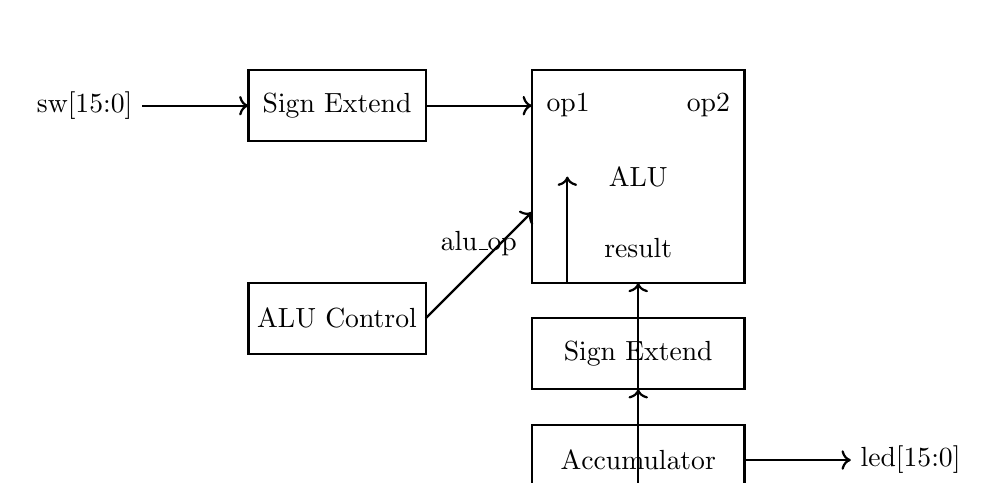
\begin{tikzpicture}[scale=0.9]
    % Sign Extend for switches
    \draw[thick] (0,4) rectangle (2.5,5);
    \node at (1.25,4.5) {Sign Extend};
    \draw[->,thick] (-1.5,4.5) -- (0,4.5);
    \node[left] at (-1.5,4.5) {sw[15:0]};
    
    % ALU
    \draw[thick] (4,2) rectangle (7,5);
    \node at (5.5,3.5) {ALU};
    \node at (5.5,4.5) {op1 \hspace{1cm} op2};
    \node at (5.5,2.5) {result};
    
    % ALU Control
    \draw[thick] (0,1) rectangle (2.5,2);
    \node at (1.25,1.5) {ALU Control};
    \draw[->,thick] (2.5,1.5) -- (4,3);
    \node[above] at (3.25,2.25) {alu\_op};
    
    % Accumulator
    \draw[thick] (4,-1) rectangle (7,0);
    \node at (5.5,-0.5) {Accumulator};
    
    % Sign Extend for accumulator
    \draw[thick] (4,0.5) rectangle (7,1.5);
    \node at (5.5,1) {Sign Extend};
    
    % Connections
    \draw[->,thick] (2.5,4.5) -- (4,4.5);
    \draw[->,thick] (5.5,0) -- (5.5,0.5);
    \draw[->,thick] (5.5,1.5) -- (5.5,2);
    \draw[->,thick] (5.5,2) -- (4.5,2) -- (4.5,3.5);
    \draw[->,thick] (5.5,2) -- (5.5,-1);
    
    % LED output
    \draw[->,thick] (7,-0.5) -- (8.5,-0.5);
    \node[right] at (8.5,-0.5) {led[15:0]};
\end{tikzpicture}
\caption{Διάγραμμα ροής της αριθμομηχανής}
\end{figure}

\subsection{Αποτελέσματα Testbench}

Η αριθμομηχανή ελέγχθηκε με τα ακόλουθα τεστ:

\begin{table}[H]
\centering
\caption{Αποτελέσματα τεστ αριθμομηχανής}
\small
\begin{tabular}{|c|c|c|c|c|c|}
\hline
\textbf{btnl,btnr,btnd} & \textbf{Acc (πριν)} & \textbf{Switches} & \textbf{Λειτουργία} & \textbf{Αναμενόμενο} & \textbf{Αποτέλεσμα} \\
\hline
Reset & xxxx & xxxx & Reset & 0x0000 & PASS \\
0,1,0 & 0x0000 & 0x285a & ADD & 0x285a & PASS \\
1,1,1 & 0x285a & 0x04c8 & XOR & 0x2c92 & PASS \\
0,0,0 & 0x2c92 & 0x0005 & SRL & 0x0164 & PASS \\
1,0,1 & 0x0164 & 0xa085 & NOR & 0x5e1a & PASS \\
1,0,0 & 0x5e1a & 0x07fe & MULT & 0x13cc & PASS \\
0,0,1 & 0x13cc & 0x0004 & SLL & 0x3cc0 & PASS \\
1,1,0 & 0x3cc0 & 0xfa65 & NAND & 0xc7bf & PASS \\
0,1,1 & 0xc7bf & 0xb2e4 & SUB & 0x14db & PASS \\
\hline
\end{tabular}
\end{table}

%==============================================================================
\section{Άσκηση 3: Register File}
%==============================================================================

\subsection{Περιγραφή}

Το Register File υλοποιεί:
\begin{itemize}
    \item 16 καταχωρητές × 32 bits (παραμετροποιήσιμο DATAWIDTH)
    \item 4 θύρες ανάγνωσης (readData1-4)
    \item 2 θύρες εγγραφής (writeData1-2)
    \item Ασύγχρονο reset (active low)
    \item Data forwarding για αποφυγή hazards
\end{itemize}

\subsection{Data Forwarding}

Σε περίπτωση που η διεύθυνση ανάγνωσης ταυτίζεται με διεύθυνση εγγραφής, δίνεται προτεραιότητα στα νέα δεδομένα:

\begin{lstlisting}[caption=Data forwarding στο Register File]
if (readReg1 == writeReg1)
    readData1 <= writeData1;
else if (readReg1 == writeReg2)
    readData1 <= writeData2;
else
    readData1 <= registers[readReg1];
\end{lstlisting}

%==============================================================================
\section{Άσκηση 4: Νευρωνικό Δίκτυο (AI Accelerator)}
%==============================================================================

\subsection{Αρχιτεκτονική Νευρωνικού}

Το νευρωνικό δίκτυο αποτελείται από 3 νευρώνες και υλοποιεί την ακόλουθη λογική:

\begin{align}
\text{inter}_1 &= \text{input}_1 >>> \text{shift\_bias}_1 \\
\text{inter}_2 &= \text{input}_2 >>> \text{shift\_bias}_2 \\
\text{inter}_3 &= \text{inter}_1 \times \text{weight}_1 + \text{bias}_1 \\
\text{inter}_4 &= \text{inter}_2 \times \text{weight}_2 + \text{bias}_2 \\
\text{inter}_5 &= \text{inter}_3 \times \text{weight}_3 + \text{inter}_4 \times \text{weight}_4 + \text{bias}_3 \\
\text{output} &= \text{inter}_5 <<< \text{shift\_bias}_3
\end{align}

\subsection{MAC Unit}

Η μονάδα MAC (Multiply and Accumulate) υλοποιεί:
\[
\text{result} = (\text{op1} \times \text{op2}) + \text{op3}
\]

Αποτελείται από δύο σειριακά συνδεδεμένες ALU:
\begin{enumerate}
    \item Πρώτη ALU: Πολλαπλασιασμός (op1 × op2)
    \item Δεύτερη ALU: Πρόσθεση (result1 + op3)
\end{enumerate}

\subsection{Finite State Machine (FSM)}

\subsubsection{Τύπος FSM: Moore}

Επιλέχθηκε \textbf{Moore FSM} για τους ακόλουθους λόγους:
\begin{itemize}
    \item Οι έξοδοι εξαρτώνται μόνο από την τρέχουσα κατάσταση
    \item Πιο εύκολη επαλήθευση και debugging
    \item Καλύτερη χρονική συμπεριφορά χωρίς glitches στις εξόδους
    \item Κατάλληλο για pipeline αρχιτεκτονικές
\end{itemize}

\subsubsection{Διάγραμμα Καταστάσεων FSM}

\begin{figure}[H]
\centering
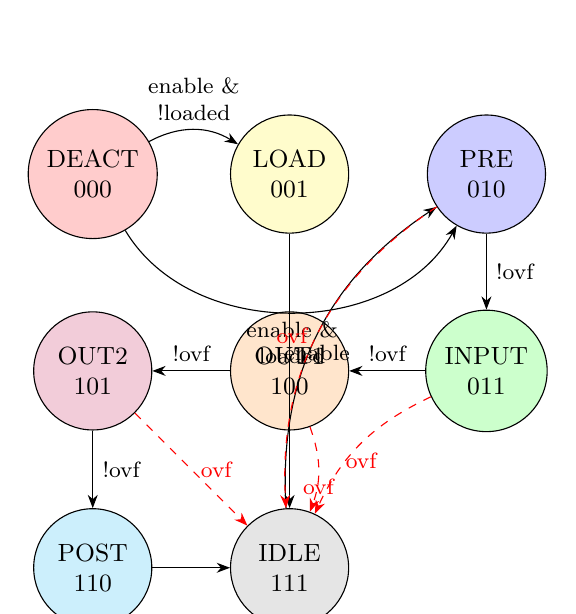
\begin{tikzpicture}[
    ->,>=Stealth,
    node distance=2.5cm,
    state/.style={circle,draw,minimum size=1.5cm,align=center,font=\small},
    every edge/.style={draw,font=\footnotesize,align=center} % align=center εδώ για να επιτρέπει \\
]
    % States
    \node[state,fill=red!20] (DEACT) {DEACT\\000};
    \node[state,fill=yellow!20] (LOAD) [right of=DEACT] {LOAD\\001};
    \node[state,fill=blue!20] (PRE) [right of=LOAD] {PRE\\010};
    \node[state,fill=green!20] (INPUT) [below of=PRE] {INPUT\\011};
    \node[state,fill=orange!20] (OUT1) [left of=INPUT] {OUT1\\100};
    \node[state,fill=purple!20] (OUT2) [left of=OUT1] {OUT2\\101};
    \node[state,fill=cyan!20] (POST) [below of=OUT2] {POST\\110};
    \node[state,fill=gray!20] (IDLE) [right of=POST] {IDLE\\111};
    
    % Transitions
    \path (DEACT) edge[bend left] node[above] {enable \&\\!loaded} (LOAD);
    \path (DEACT) edge[bend right=60] node[below] {enable \&\\loaded} (PRE);
    \path (LOAD) edge node[above] {} (IDLE);
    \path (PRE) edge node[right] {!ovf} (INPUT);
    \path (INPUT) edge node[above] {!ovf} (OUT1);
    \path (OUT1) edge node[above] {!ovf} (OUT2);
    \path (OUT2) edge node[right] {!ovf} (POST);
    \path (POST) edge node[above] {} (IDLE);
    \path (IDLE) edge[bend left] node[below] {enable} (PRE);
    
    % Overflow transitions
    \path (PRE) edge[bend right=30,dashed,red] node[left] {ovf} (IDLE);
    \path (INPUT) edge[bend right=20,dashed,red] node[below] {ovf} (IDLE);
    \path (OUT1) edge[bend left=20,dashed,red] node[below] {ovf} (IDLE);
    \path (OUT2) edge[dashed,red] node[right] {ovf} (IDLE);
\end{tikzpicture}
\caption{Διάγραμμα καταστάσεων FSM του νευρωνικού (κόκκινες διακεκομμένες: overflow transitions)}
\end{figure}

\subsubsection{Περιγραφή Καταστάσεων}

\begin{table}[H]
\centering
\caption{Καταστάσεις FSM}
\begin{tabular}{|c|c|p{8cm}|}
\hline
\textbf{Κατάσταση} & \textbf{Κωδικός} & \textbf{Περιγραφή} \\
\hline
DEACTIVATED & 000 & Αρχική κατάσταση, αναμονή για enable \\
LOAD\_WEIGHTS & 001 & Φόρτωση βαρών/πολώσεων από ROM σε RegFile \\
PREPROCESS & 010 & Αριθμητική ολίσθηση δεξιά στις εισόδους \\
INPUT\_LAYER & 011 & Εκτέλεση νευρώνων 1 και 2 (παράλληλα) \\
OUTPUT\_LAYER1 & 100 & Πολλαπλασιασμοί για νευρώνα 3 \\
OUTPUT\_LAYER2 & 101 & Προσθέσεις για νευρώνα 3 \\
POSTPROCESS & 110 & Αριθμητική ολίσθηση αριστερά στην έξοδο \\
IDLE & 111 & Αναμονή για νέες εισόδους \\
\hline
\end{tabular}
\end{table}

\subsection{Χειρισμός Υπερχείλισης}

Σε περίπτωση overflow σε οποιοδήποτε στάδιο:
\begin{enumerate}
    \item Το FSM μεταβαίνει άμεσα στην κατάσταση IDLE
    \item Η έξοδος τίθεται στον μέγιστο θετικό αριθμό (0x7FFFFFFF)
    \item Το σήμα \texttt{total\_ovf} ενεργοποιείται
    \item Το \texttt{ovf\_fsm\_stage} δείχνει το στάδιο όπου συνέβη η υπερχείλιση
\end{enumerate}

\subsection{Αποθήκευση Δεδομένων}

Επιλέχθηκε η χρήση \textbf{ενδιάμεσων registers} αντί για αποθήκευση στο Register File για τους εξής λόγους:
\begin{itemize}
    \item Μείωση της πολυπλοκότητας πρόσβασης στο RegFile
    \item Αποφυγή conflicts με τις θύρες ανάγνωσης/εγγραφής
    \item Καλύτερη απόδοση λόγω άμεσης πρόσβασης
    \item Το RegFile χρησιμοποιείται μόνο για τα βάρη και τις πολώσεις
\end{itemize}

\subsection{Testbench Νευρωνικού}

Το testbench εκτελεί 100 επαναλήψεις με 3 τεστ ανά επανάληψη:
\begin{enumerate}
    \item \textbf{Κανονικό εύρος:} [-4096, 4095]
    \item \textbf{Θετικό overflow:} [MAX\_POS/2, MAX\_POS]
    \item \textbf{Αρνητικό overflow:} [MAX\_NEG, MAX\_NEG/2]
\end{enumerate}

Η συνάρτηση αναφοράς \texttt{nn\_model} υπολογίζει το αναμενόμενο αποτέλεσμα για σύγκριση.

%==============================================================================
\section{Κυματομορφές Προσομοίωσης}
%==============================================================================

\subsection{Κυματομορφές Αριθμομηχανής (Άσκηση 2)}

\begin{figure}[H]
\centering
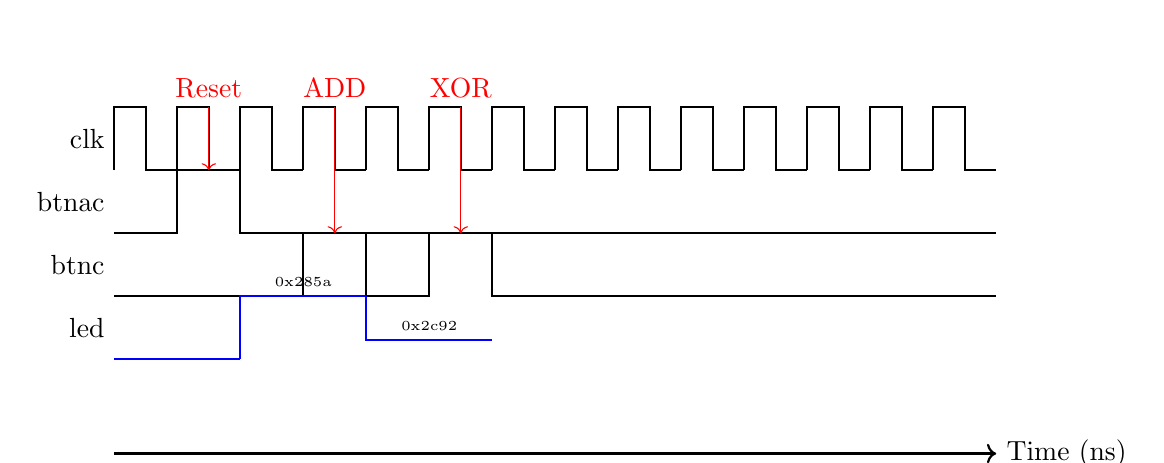
\begin{tikzpicture}[scale=0.8]
    % Time axis
    \draw[->,thick] (0,0) -- (14,0) node[right] {Time (ns)};
    
    % Clock
    \node[left] at (0,5) {clk};
    \foreach \i in {0,1,2,3,4,5,6,7,8,9,10,11,12,13} {
        \draw[thick] (\i,4.5) -- (\i,5.5) -- (\i+0.5,5.5) -- (\i+0.5,4.5) -- (\i+1,4.5);
    }
    
    % btnac
    \node[left] at (0,4) {btnac};
    \draw[thick] (0,3.5) -- (1,3.5) -- (1,4.5) -- (2,4.5) -- (2,3.5) -- (14,3.5);
    
    % btnc
    \node[left] at (0,3) {btnc};
    \draw[thick] (0,2.5) -- (3,2.5) -- (3,3.5) -- (4,3.5) -- (4,2.5) -- 
                 (5,2.5) -- (5,3.5) -- (6,3.5) -- (6,2.5) -- (14,2.5);
    
    % led
    \node[left] at (0,2) {led};
    \draw[thick,blue] (0,1.5) -- (2,1.5);
    \draw[thick,blue] (2,1.5) -- (2,2.5) -- (4,2.5);
    \node[above,font=\tiny] at (3,2.5) {0x285a};
    \draw[thick,blue] (4,2.5) -- (4,1.8) -- (6,1.8);
    \node[above,font=\tiny] at (5,1.8) {0x2c92};
    
    % Annotations
    \draw[<-,red] (1.5,4.5) -- (1.5,5.5) node[above] {Reset};
    \draw[<-,red] (3.5,3.5) -- (3.5,5.5) node[above] {ADD};
    \draw[<-,red] (5.5,3.5) -- (5.5,5.5) node[above] {XOR};
\end{tikzpicture}
\caption{Σχηματική αναπαράσταση κυματομορφών αριθμομηχανής}
\end{figure}

\textbf{Σημείωση:} Για λεπτομερείς κυματομορφές, χρησιμοποιήστε τα αρχεία VCD που παράγονται από τα testbenches στο Playground EDA.

\subsection{Κυματομορφές Νευρωνικού (Άσκηση 4)}

\begin{figure}[H]
\centering
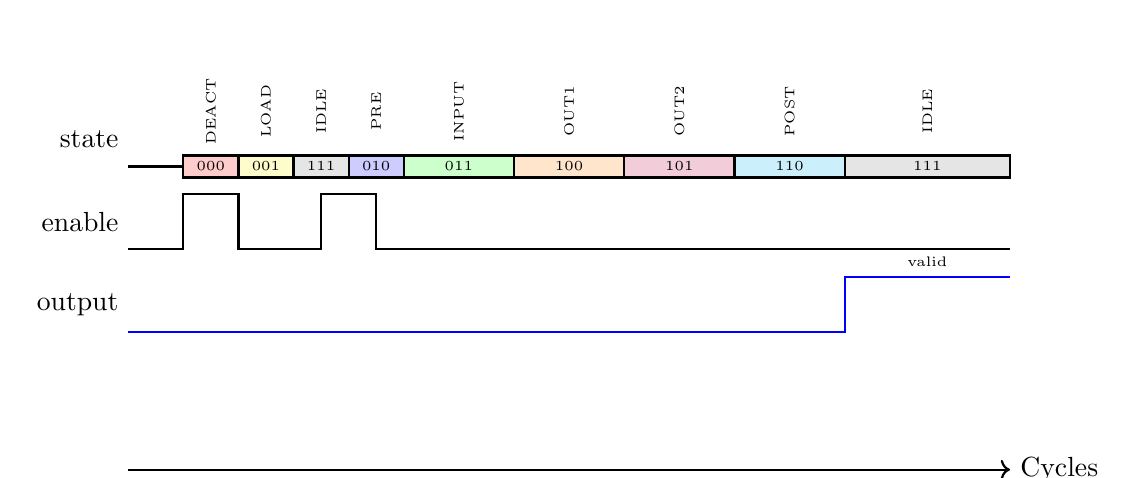
\begin{tikzpicture}[scale=0.7]
    % Time axis
    \draw[->,thick] (0,0) -- (16,0) node[right] {Cycles};
    
    % FSM State
    \node[left] at (0,6) {state};
    \draw[thick] (0,5.5) -- (1,5.5);
    \draw[thick,fill=red!20] (1,5.3) rectangle (2,5.7);
    \node[font=\tiny] at (1.5,5.5) {000};
    \draw[thick,fill=yellow!20] (2,5.3) rectangle (3,5.7);
    \node[font=\tiny] at (2.5,5.5) {001};
    \draw[thick,fill=gray!20] (3,5.3) rectangle (4,5.7);
    \node[font=\tiny] at (3.5,5.5) {111};
    \draw[thick,fill=blue!20] (4,5.3) rectangle (5,5.7);
    \node[font=\tiny] at (4.5,5.5) {010};
    \draw[thick,fill=green!20] (5,5.3) rectangle (7,5.7);
    \node[font=\tiny] at (6,5.5) {011};
    \draw[thick,fill=orange!20] (7,5.3) rectangle (9,5.7);
    \node[font=\tiny] at (8,5.5) {100};
    \draw[thick,fill=purple!20] (9,5.3) rectangle (11,5.7);
    \node[font=\tiny] at (10,5.5) {101};
    \draw[thick,fill=cyan!20] (11,5.3) rectangle (13,5.7);
    \node[font=\tiny] at (12,5.5) {110};
    \draw[thick,fill=gray!20] (13,5.3) rectangle (16,5.7);
    \node[font=\tiny] at (14.5,5.5) {111};
    
    % Enable
    \node[left] at (0,4.5) {enable};
    \draw[thick] (0,4) -- (1,4) -- (1,5) -- (2,5) -- (2,4) --
                 (3.5,4) -- (3.5,5) -- (4.5,5) -- (4.5,4) -- (16,4);
    
    % final_output
    \node[left] at (0,3) {output};
    \draw[thick,blue] (0,2.5) -- (13,2.5) -- (13,3.5) -- (16,3.5);
    \node[above,font=\tiny] at (14.5,3.5) {valid};
    
    % Annotations
    \node[font=\tiny,rotate=90] at (1.5,6.5) {DEACT};
    \node[font=\tiny,rotate=90] at (2.5,6.5) {LOAD};
    \node[font=\tiny,rotate=90] at (3.5,6.5) {IDLE};
    \node[font=\tiny,rotate=90] at (4.5,6.5) {PRE};
    \node[font=\tiny,rotate=90] at (6,6.5) {INPUT};
    \node[font=\tiny,rotate=90] at (8,6.5) {OUT1};
    \node[font=\tiny,rotate=90] at (10,6.5) {OUT2};
    \node[font=\tiny,rotate=90] at (12,6.5) {POST};
    \node[font=\tiny,rotate=90] at (14.5,6.5) {IDLE};
\end{tikzpicture}
\caption{Σχηματική αναπαράσταση κυματομορφών FSM νευρωνικού}
\end{figure}

%==============================================================================
\section{Συμπεράσματα}
%==============================================================================

Η εργασία ολοκληρώθηκε επιτυχώς με τα ακόλουθα αποτελέσματα:

\begin{enumerate}
    \item \textbf{ALU (alu.v):} Υλοποιήθηκε 32-bit ALU με 12 λειτουργίες και ανίχνευση υπερχείλισης
    \item \textbf{Αριθμομηχανή (calc.v, calc\_enc.v):} Λειτουργική αριθμομηχανή με structural encoder
    \item \textbf{Register File (regfile.v):} 16×32-bit με data forwarding
    \item \textbf{Νευρωνικό (mac\_unit.v, nn.v):} Moore FSM με 7 καταστάσεις και χειρισμό overflow
\end{enumerate}

Τα testbenches επιβεβαίωσαν την ορθή λειτουργία όλων των κυκλωμάτων.

%==============================================================================
\section{Αναφορές}
%==============================================================================

\begin{enumerate}
    \item ECEN 323: Computer Organization, BYU ECE. Διαθέσιμο: \url{https://ecen323wiki.groups.et.byu.net/}
    \item IEEE Standard for Verilog Hardware Description Language (IEEE 1364-2005)
    \item Playground EDA - Online Verilog Simulator
\end{enumerate}

%==============================================================================
\section*{Παράρτημα: Λίστα Αρχείων}
%==============================================================================

\begin{table}[H]
\centering
\begin{tabular}{|l|l|}
\hline
\textbf{Αρχείο} & \textbf{Περιγραφή} \\
\hline
alu.v & Αριθμητική/Λογική Μονάδα 32-bit \\
calc.v & Module αριθμομηχανής \\
calc\_enc.v & Encoder για alu\_op (structural) \\
calc\_tb.v & Testbench αριθμομηχανής \\
regfile.v & Register File 16×32-bit \\
mac\_unit.v & Multiply-Accumulate Unit \\
nn.v & Νευρωνικό δίκτυο με FSM \\
tb\_nn.v & Testbench νευρωνικού \\
\hline
\end{tabular}
\caption{Λίστα αρχείων εργασίας}
\end{table}

\end{document}